%%%%%%%%%%%%%%%%%%%%%%%%%%%%%%%%%%%%%%%%%
% a0poster Landscape Poster
% LaTeX Template
% Version 1.0 (22/06/13)
%
% The a0poster class was created by:
% Gerlinde Kettl and Matthias Weiser (tex@kettl.de)
% 
% This template has been downloaded from:
% http://www.LaTeXTemplates.com
%
% License:
% CC BY-NC-SA 3.0 (http://creativecommons.org/licenses/by-nc-sa/3.0/)
%
%%%%%%%%%%%%%%%%%%%%%%%%%%%%%%%%%%%%%%%%%

%----------------------------------------------------------------------------------------
%	PACKAGES AND OTHER DOCUMENT CONFIGURATIONS
%----------------------------------------------------------------------------------------

\documentclass[a0,landscape]{a0poster}

\usepackage{multicol} % This is so we can have multiple columns of text side-by-side
\columnsep=100pt % This is the amount of white space between the columns in the poster
\columnseprule=3pt % This is the thickness of the black line between the columns in the poster

\usepackage[svgnames]{xcolor} % Specify colors by their 'svgnames', for a full list of all colors available see here: http://www.latextemplates.com/svgnames-colors

\usepackage{times} % Use the times font
%\usepackage{palatino} % Uncomment to use the Palatino font

\usepackage{graphicx} % Required for including images
\graphicspath{{figures/}} % Location of the graphics files
\usepackage{booktabs} % Top and bottom rules for table
\usepackage[font=small,labelfont=bf]{caption} % Required for specifying captions to tables and figures
\usepackage{amsfonts, amsmath, amsthm, amssymb} % For math fonts, symbols and environments
\usepackage{wrapfig} % Allows wrapping text around tables and figures
\usepackage{mathrsfs}
\usepackage{tikz-cd}
\usepackage{here}
\usepackage{mathtools}
\usepackage{color}
\usepackage{titlesec}
\usepackage{adjustbox}
\usepackage{tcolorbox}
\tcbuselibrary{breakable, skins, theorems}
\tcbset{nobeforeafter}

\renewcommand{\theenumi}{\arabic{enumi}}
\renewcommand{\labelenumi}{(\theenumi) }
\providecommand{\MR}{\relax\ifhmode\unskip\space\fi MR }
%% Theorems
\theoremstyle{plain}

\newtheorem{theorem}{Theorem}[section]
\newtheorem{conjecture}[theorem]{Conjecture}
\newtheorem{lemma}[theorem]{Lemma}
\newtheorem{proposition}[theorem]{Proposition}
\newtheorem{corollary}[theorem]{Corollary}

\theoremstyle{definition}
\newtheorem{definition}[theorem]{Definition}
\newtheorem{example}[theorem]{Example}
\newtheorem{remark}[theorem]{Remark}

%% Some operators
\DeclareMathOperator{\Hom}{\mathrm{Hom}}
\DeclareMathOperator{\Tor}{\mathrm{Tor}}
\DeclareMathOperator{\CHom}{\mathcal{H}\!\mathit{om}}
\DeclareMathOperator{\CTor}{\mathcal{T}\!\mathit{or}}
\DeclareMathOperator{\Auteq}{\mathrm{Auteq}}
\DeclareMathOperator{\Cone}{\mathrm{Cone}}
\DeclareMathOperator{\ev}{\mathrm{ev}}
\DeclareMathOperator{\id}{\mathrm{id}}
\DeclareMathOperator{\depth}{\mathrm{depth}}
\DeclareMathOperator{\Pic}{\mathrm{Pic}}
\DeclareMathOperator{\MCG}{\mathrm{MCG}}
\DeclareMathOperator{\PMCG}{\mathrm{PMCG}}
\DeclareMathOperator{\RHom}{\mathrm{RHom}}
\DeclareMathOperator{\Ker}{\mathrm{Ker}}
\DeclareMathOperator{\Image}{\mathrm{Im}}
\DeclareMathOperator{\Aut}{\mathrm{Aut}}
\DeclareMathOperator{\Inn}{\mathrm{Inn}}
\DeclareMathOperator{\Out}{\mathrm{Out}}
\DeclareMathOperator{\Supp}{\mathrm{Supp}}
\DeclareMathOperator{\SL}{\mathrm{SL}}
\DeclareMathOperator{\Spec}{\mathrm{Spec}}
\DeclareMathOperator{\Perf}{\mathrm{Perf}}
\DeclareMathOperator{\NS}{\mathrm{NS}}
\DeclareMathOperator{\Ext}{\mathrm{Ext}}
\DeclareMathOperator{\Hilb}{\mathrm{Hilb}}
\DeclareMathOperator{\res}{\mathrm{res}}

\newcommand{\nc}{\newcommand}

%% Calligraphic letters

\nc{\cF}{{\mathcal{F}}}
\nc{\cG}{{\mathcal{G}}}
\nc{\cH}{{\mathcal{H}}}

\nc{\cO}{{\mathcal{O}}}
\nc{\cU}{{\mathcal{U}}}
\nc{\cW}{{\mathcal{W}}}

%% Blackboard letters
\nc{\bA}{{\mathbb{A}}}
\nc{\bC}{{\mathbb{C}}}
\nc{\bP}{{\mathbb{P}}}
\nc{\bQ}{{\mathbb{Q}}}
\nc{\bZ}{{\mathbb{Z}}}

%% Script letters
\nc{\sT}{{\mathscr{T}}}

\titleformat*{\section}{\LARGE\bfseries}
\titleformat*{\subsection}{\Large\bfseries}
\begin{document}

%----------------------------------------------------------------------------------------
%	POSTER HEADER 
%----------------------------------------------------------------------------------------

% The header is divided into three boxes:
% The first is 55% wide and houses the title, subtitle, names and university/organization
% The second is 25% wide and houses contact information
% The third is 19% wide and houses a logo for your university/organization or a photo of you
% The widths of these boxes can be easily edited to accommodate your content as you see fit

\begin{minipage}{\linewidth}
    \centering{
        \veryHuge \color{NavyBlue} \textbf{Half-spherical twists on derived categories of coherent sheaves} \color{Black}\\ % Title
        \Huge\text{based on arXiv:2302.12501}\\[1cm] % Subtitle
        \Huge \textbf{Hayato Arai} \\ % Author(s)
        \huge  Graduate School of Mathematical Sciences,
        The University of Tokyo\\ % University/organization
        %email: hayato@ms.u-tokyo.ac.jp
    }
\end{minipage}

% %
% \begin{minipage}[b]{0.25\linewidth}
%     \color{DarkSlateGray}\Large \textbf{Contact Information:}\\
%     Department Name\\ % Address
%     University Name\\
%     123 Broadway, State, Country\\\\
%     Phone: +1 (000) 111 1111\\ % Phone number
%     Email: \texttt{john@LaTeXTemplates.com}\\ % Email address
% \end{minipage}
% %
% \begin{minipage}[b]{0.19\linewidth}
%     
\includegraphics[width=20cm]{logo.png} % Logo or a photo of you, adjust its dimensions here
% \end{minipage}

\vspace{2cm} % A bit of extra whitespace between the header and poster content

%----------------------------------------------------------------------------------------
\large
\begin{multicols}{3} % This is how many columns your poster will be broken into, a poster with many figures may benefit from less columns whereas a text-heavy poster benefits from more

    %----------------------------------------------------------------------------------------
    %	ABSTRACT
    %----------------------------------------------------------------------------------------

    % \color{Navy} % Navy color for the abstract

    %----------------------------------------------------------------------------------------
    %	INTRODUCTION
    %----------------------------------------------------------------------------------------

    %\color{SaddleBrown} % SaddleBrown color for the introduction

    \color{NavyBlue}\section{Introduction}

    \color{DarkSlateGray} % DarkSlateGray color for the rest of the content
    \subsection{Mirror symmetry for singular fibers of type $\textrm{I}_n$ of elliptic surfaces}
    Let $\pi \colon S \to C$ be a relatively minimal, smooth projective elliptic surface.
    The possible singular fibers of $\pi$ are classified by Kodaira and N\'{e}ron.
    Among them, \textit{the singular fiber of type $\textrm{I}_n$} is the cyclic configuration of $n$ smooth rational curves.

    Lekili and Polishchuk \cite{MR3663596} established mirror symmetry between the type $\textrm{I}_n$ singular fiber $Y_n$ and the $n$-punctured torus $T_n$, i.e.~ they showed that the derived category $D^b(Y_n)$ of coherent sheaves on $Y_n$ and the wrapped Fukaya category $D^\pi(\mathcal{W}(T_n))$ of $T_n$ are equivalent.

    For example, the equivalence includes the following correspondence of objects, where $G_i$'s are irreducible components and $\gamma_F$ denotes the corresponding curve to the object $F \in D^b(Y_n)$:
    \begin{center}
        \centering
        \begin{displaymath}
            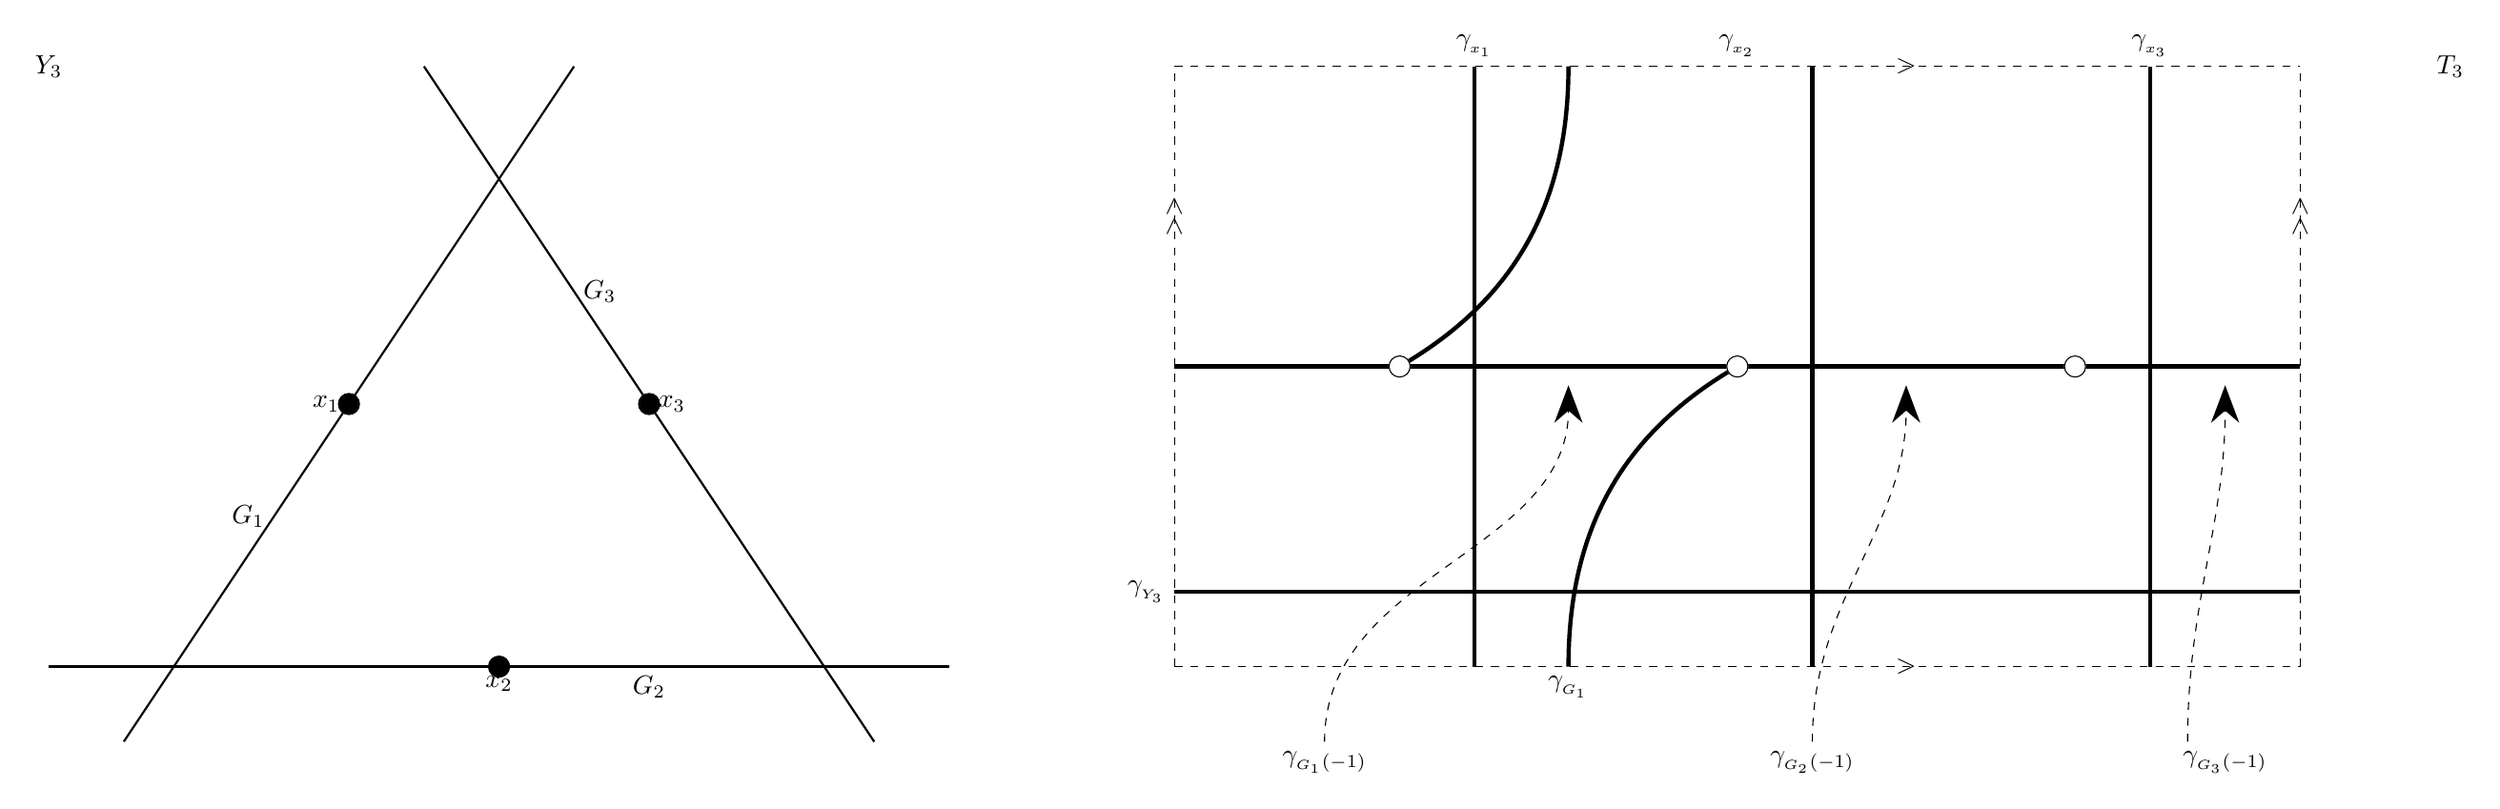
\begin{tikzpicture}
                % fiber
                \draw(-10, 8) node{$Y_3$};
                \draw[thick] (-9,-1)--(-3,8);
                \draw[thick] (-10,0)--(2,0);
                \draw[thick] (1,-1)--(-5,8);

                % points
                \filldraw[black] (-6, 3.5) circle (4pt);
                \filldraw[black] (-4, 0) circle (4pt);
                \filldraw[black] (-2, 3.5) circle (4pt);

                \draw(-6, 3.5) node[left]{$x_1$};
                \draw(-4, 0) node[below]{$x_2$};
                \draw(-2, 3.5) node[right]{$x_3$};

                % components
                \draw(-7, 2) node[left]{$G_1$};
                \draw(-2, 0) node[below]{$G_2$};
                \draw(-3, 5) node[right]{$G_3$};

                % big square
                \draw(22, 8) node{$T_3$};
                \draw[dashed] (5,0)--(20,0);
                \draw(14.75, 0) node{$>$};
                \draw[dashed] (5,0)--(5,8);
                \draw(5, 6) node{\rotatebox{90}{$>>$}};
                \draw[dashed] (5,8)--(20,8);
                \draw(14.75, 8) node{$>$};
                \draw[dashed] (20,0)--(20,8);
                \draw(20, 6) node{\rotatebox{90}{$>>$}};

                % horizontal lines
                \draw[ultra thick] (5, 1)--(20, 1);
                \draw[ultra thick] (5, 4)--(20, 4);
                \draw(5, 1) node[left]{$\gamma_{\cO_{Y_3}}$};
                % \draw[thick] (3, 2)--(5, 2);
                % \draw[thick] (9, 2)--(11, 2);

                % \draw[thick] (0, 0.5)--(11, 0.5);

                % vertical lines
                \draw[ultra thick] (8+1, 0)--(8+1, 8);
                \draw(8+1, 8) node[above]{$\gamma_{\cO_{x_1}}$};
                \draw[ultra thick] (12.5+1, 0)--(12.5+1, 8);
                \draw(12.5, 8) node[above]{$\gamma_{\cO_{x_2}}$};
                \draw[ultra thick] (17+1, 0)--(17+1, 8);
                \draw(17+1, 8) node[above]{$\gamma_{\cO_{x_3}}$};

                % curves 
                \draw[ultra thick] (8, 4) to[out=30,in=-90] (10.25, 8);
                \draw[ultra thick] (10.25, 0) to[out=90,in=-150] (12.5, 4);
                \draw(10.25, 0) node[below]{$\gamma_{\cO_{G_1}}$};
                % punctures
                \foreach \u in {8, 12.5, 17}
                    {
                        \filldraw[white] (\u, 4) circle (4pt);
                        \draw[black] (\u, 4) circle (4pt);
                    }

                % O_G(-1)
                \draw[dashed, -{Stealth[length=5mm]}] (7, -1) to[out=90, in=-90] (10.25, 3.75);
                \draw(7, -1) node[below]{$\gamma_{\cO_{G_1}(-1)}$};
                \draw[dashed, -{Stealth[length=5mm]}] (13.5, -1) to[out=90, in=-90] (14.75, 3.75);
                \draw(13.5, -1) node[below]{$\gamma_{\cO_{G_2}(-1)}$};
                \draw[dashed, -{Stealth[length=5mm]}] (18.5, -1) to[out=90, in=-90] (19, 3.75);
                \draw(19, -1) node[below]{$\gamma_{\cO_{G_3}(-1)}$};

                % % notations
                % \draw(0, 0.5) node[left]{$\gamma_{\cO_Y}$};
                % \draw(2, 4) node[above]{$\gamma_{\cO_{x_1}}$};
                % \draw(4, 4) node[above]{$\gamma_{\cO_{x_2}}$};
                % \draw(10, 4) node[above]{$\gamma_{\cO_{x_n}}$};

                % \draw(2, 3) node[above left]{$\gamma_{\cO_{G_1}(-1)}$};
                % \draw(1, 3) to[out=-90,in=135](1.5, 2);
                % \draw(4, 3) node[above left]{$\gamma_{\cO_{G_2}(-1)}$};
                % \draw(3, 3) to[out=-90,in=135](3.5, 2);

                % \draw(11, 2) node[right]{$\gamma_{\cO_{G_n}(-1)}$};

            \end{tikzpicture}
        \end{displaymath}
        \captionof{figure}{\color{NavyBlue} The correspondence of objects via $D^b(Y_n) \simeq D^\pi(\mathcal{W}(T_n))$, $n=3$.}
    \end{center}


    Combining this with the theory of topological Fukaya categories of surfaces developed by Haiden, Katzarkov, and Kontsevich \cite{MR3735868}, Opper \cite{2020arXiv201108288O} described the autoequivalence group of $D^b(Y_n)$ with the following exact sequence:
    \begin{tcolorbox}[
            colback = blue!10!white,
            colframe = blue!10!white,
            fonttitle = \bfseries,
            breakable = true]
        \begin{equation*}
            1 \to (\bC^\times)^n \times \bZ[1] \times \Pic^0(Y_n) \to \Auteq{D^b(Y_n)} \xrightarrow{\Upsilon} \MCG(T_n) \to 1.
        \end{equation*}
    \end{tcolorbox}

    Here $\MCG(T_n)$ denotes the mapping class group of $T_n$ and the morphism $\Upsilon$ is induced by the equivalence $D^b(Y_n) \simeq D^\pi(\mathcal{W}(T_n))$.
    %----------------------------------------------------------------------------------------
    %	MATERIALS AND METHODS
    %----------------------------------------------------------------------------------------
    \subsection{Autoequivalences of elliptic surfaces}

    %Let $\pi \colon S \to C$ be a relatively minimal, smooth projective elliptic surface.
    Uehara \cite{MR3568337} gave the following description of the autoequivalence group $\Auteq D^b(S)$.
    This result implies that the study of the structure of $\Auteq D^b(S)$ reduces to that of $B$.

    \begin{tcolorbox}[
            colback = blue!10!white,
            colframe = blue!10!white,
            fonttitle = \bfseries,
            breakable = true]
        \begin{theorem}
            \quad
            \begin{itemize}
                \item $S$ has non-zero Kodaira dimension
                \item all singular fibers of $\pi$ are non-multiple and of type $\rm{I}_n$, $n \geq 2$
                \item  $B = \langle T_{\cO_G(a)} \mid G \subset S \text{ : an irreducible component of a singular fiber, } a \in \bZ \rangle$: the subgroup of $\Auteq D^b(S)$ generated by twist functors $T_{\cO_G(a)}$, where $\cO_G(a)$ is the line bundle of degree $a$ on $G \simeq \bP^1$
            \end{itemize}

            Then there is the exact sequence
            \begin{align*}
                1 \to \langle B, (-)\otimes \cO_S(D)\mid D.F=0, F \textrm{ is a fiber } \rangle & \rtimes \Aut{S} \times \bZ[2]      \\
                                                                                                & \to \Auteq{D^b(S)} \to \SL(2,\bZ).
            \end{align*}
        \end{theorem}
    \end{tcolorbox}



    \color{Green}
    \subsection{Main results}
    \color{DarkSlateGray}
    We study the group $B$ in terms of the mapping class group of the $n$-punctured torus so that we reveal the whole structure of $\Auteq D^b(S)$.
    \begin{enumerate}
        \item\leavevmode %<--------------
        \adjustbox{valign=t}{%
            \begin{tcolorbox}[
                    %width=0.934\textwidth,
                    colback={green!10!white},
                    colframe = green!10!white,
                    fonttitle = \bfseries,
                    breakable = true
                ]We construct a natural ``restriction'' morphism $\res \colon B \to \Auteq{D^b(F)}$ for each fiber $F$, which is nontrivial if $F$ is a reducible fiber.
            \end{tcolorbox}
        }
        \item Combining with mirror symmetry for the singular fibers of type $\textrm{I}_n$, we have the exact sequences
              \begin{tcolorbox}[
                      colback = green!10!white,
                      colframe = green!10!white,
                      fonttitle = \bfseries,
                      breakable = true]
                  \begin{equation*}
                      1 \to \langle (-)\otimes \cO_S(Y_{n_j}) \mid 1 \leq j \leq m\rangle \to B \xrightarrow{\Upsilon \circ \, \res} \prod_{j=1}^m \MCG(T_{n_j}),
                  \end{equation*}\end{tcolorbox}
              where $Y_{n_j}$ is the singular fiber of type $\textrm{I}_{n_j}$ and $\{Y_{n_j}\}_{j=1}^m$ is the set of all singular fibers of $S$.

        \item For $G \subset Y_{n}$, $a \in \bZ$, and the curve $\gamma_{\cO_G(a)}$ on $T_{n}$ corresponding to $\cO_{G}(a)$ under the equivalence $D^b(Y_n) \simeq D^\pi(\mathcal{W}(T_n))$, \color{black}\colorbox{green!10!white}{the twist functor $T_{\cO_G(a)} \in B$ is mapped} \colorbox{green!10!white}{to \textit{the half twist along $\gamma_{\cO_G(a)}$} in $\MCG(T_n) \subset \prod_{j=1}^m \MCG(T_{n_j})$.}\color{DarkSlateGray}
        \item The image of $\Upsilon \circ \res$ is generated by the half twists along the finite number of curves $\{\gamma_{\cO_G}, \gamma_{\cO_G(-1)} \mid G \subset Y_{n_j}\text{: an irreducible component, } 1 \leq j \leq m \}$.
    \end{enumerate}

    \begin{center}
        \centering
        \begin{displaymath}
            \begin{tikzpicture}[scale=2.5]
                \draw (0, 1.5) circle[radius=1.5];
                \draw[thick] (-0.5, 1.5)--(0.5, 1.5);
                \draw(0, 1.5) node{$>$};
                \draw[dashed] (-1.5, 1.5)--(-0.5, 1.5);
                \draw[dashed] (0.5, 1.5)--(1.5, 1.5);

                \foreach \u in {-0.5, 0.5}
                    {
                        \filldraw[white] (\u, 1.5) circle (2pt);
                        \draw[black] (\u, 1.5) circle (2pt);
                    }
                \draw(0, 1.5) node[above]{$\gamma$};

                \draw(2.5, 1.5) node{$\rightarrow$};

                \draw (0+5, 1.5) circle[radius=1.5];
                \draw[thick] (-0.5+5, 1.5)--(0.5+5, 1.5);
                \draw(5, 1.5) node{$<$};


                \draw[dashed](-1.5+5, 1.5) to[out=-30,in=180](-0.5+5, 0.75);
                \draw[dashed](-0.5+5, 0.75) to[out=0,in=-90](0.5+5, 1.5);

                \draw[dashed](-0.5+5, 1.5) to[out=90,in=180](0.5+5, 2.25);
                \draw[dashed](0.5+5, 2.25) to[out=0,in=150](1.5+5, 1.5);


                \foreach \u in {-0.5, 0.5}
                    {
                        \filldraw[white] (\u+5, 1.5) circle (2pt);
                        \draw[black] (\u+5, 1.5) circle (2pt);
                    }
            \end{tikzpicture}
        \end{displaymath}
        \captionof{figure}{\color{NavyBlue} The half twist along the curve $\gamma$.}
    \end{center}


    \color{NavyBlue}\section{Sketch of the proof}

    \color{DarkSlateGray}
    We provide a sketch of the proofs of the result (1) and (3).
    \subsection{Result (1)}
    We prepare the following theorem to prove the result (1). This is a generalization of the relation between twist functors and $\bP$-twists by Huybrechts and Thomas.


    \begin{theorem}
        \quad
        \begin{itemize}
            \item $\pi \colon X \to T$ : a flat morphism between smooth quasi-projective varieties
            \item $i \colon Y = \pi^{-1}(0) \hookrightarrow X$ : the fiber at $0 \in T$
            \item $E \in D^b(Y)$ : an object such that $i_* E \in D^b(X)$ is a spherical object
            \item $T_{i_* E} \in \Auteq D^b(X)$ : the corresponding twist functor
        \end{itemize}
        Then there is a unique $H_E \in \Auteq D^b(Y)$ which makes the following diagram commutative:
        \begin{equation} \label{eq:cd2}
            \begin{tikzcd}
                D^b(Y) \arrow[r,"i_*"]\arrow[d, "H_E"'] & D^b(X) \arrow[d,"T_{i_* E}"]\\
                D^b(Y) \arrow[r, "i_*"]& D^b(X).
            \end{tikzcd}
        \end{equation}
    \end{theorem}


    \begin{tcolorbox}[
            colback = green!10!white,
            colframe = green!10!white,
            fonttitle = \bfseries,
            breakable = true]
        \begin{proof}[Proof of the result (1)]
            The uniqueness and the construction of $H_E$ ensure that we have a well-defined morphism $\res \colon B \to \Auteq D^b(F)$ such that $\res(T_{\cO_G(a)}) = H_{\cO_G(a)}$ if $G \subset F$ and $\res(T_{\cO_G(a)}) = \id$ otherwise.
        \end{proof}
    \end{tcolorbox}
    \subsection{Result (3)}
    For the proof of the result (3), we use the following three facts.
    \begin{itemize}
        \item The group $\pi_1(T_{n})$ is generated by the curves $\gamma_{\cO_{Y_n}}, \gamma_{\cO_{x_1}}, \dots, \gamma_{\cO_{x_{n}}}$ (see Figure 1).
        \item An element of $\MCG(T_{n})$ is determined by its action on $\pi_1(T_{n})$ (Dehn--Nielsen--Baer theorem).
              \item{\cite{MR3735868, 2020arXiv201108288O}} There are correspondences between indecomposable objects of $D^b(Y_{n})$ and homotopy classes of curves on $T_{n}$ ($+$ some data), and between dimensions of $\Hom$-spaces in $D^b(Y_{n})$ and intersection numbers of curves on $T_{n}$.
    \end{itemize}

    \begin{tcolorbox}[
            colback = green!10!white,
            colframe = green!10!white,
            fonttitle = \bfseries,
            breakable = true]
        \begin{proof}[Proof of the result (3)]
            For simplicity, we assume that $x_1 \in G$ and $a = 0$.
            We denote the image under the morphism $\Upsilon \circ \res$ of the twist functor $T_{\cO_{G}}$ by $H$, and the half twist along $\gamma_{\cO_G}$ by $H'$.

            Given the first and second facts, we only need to check the identities $H(\gamma_{\cO_{Y_n}})=H'(\gamma_{\cO_{Y_n}}), H(\gamma_{\cO_{x_1}})=H'(\gamma_{\cO_{x_1}}), \dots, H(\gamma_{\cO_{x_n}})=H'(\gamma_{\cO_{x_n}})$ of curves.

            Next, due to the construction of $\Upsilon$ and $\res$, the curve $H(\gamma_{\cO_{Y_n}})$ on $T_n$ (resp. $H(\gamma_{\cO_{x_i}})$) corresponds to the object $H_{\cO_G}(\cO_{Y_n}) \in D^b(Y_n)$ (resp. $H_{\cO_G}(\cO_{x_i})$) under the third fact.

            Finally, these correspondences and the third fact enable us to compute some intersection numbers between $H(\gamma_{\cO_{Y_n}})$ (or $H(\gamma_{\cO_{x_i}})$) and other curves using basic computations in homological algebra.
            We can collect enough intersection numbers to determine the curves $H(\gamma_{\cO_{Y_n}})$ and $H(\gamma_{\cO_{x_i}})$, and this finishes the proof.
        \end{proof}
    \end{tcolorbox}
    % \begin{theorem}
    %     \quad
    %     \begin{itemize}
    %         \item $\pi \colon S \to C$ : a relatively minimal, smooth projective elliptic surface
    %         \item all reducible fibers $\{Y_j\}_{j = 1}^m$ are non-multiple and of type $\textrm{I}$
    %         \item $n_j \geq 2$ : the number of irreducible components of $Y_j$
    %         \item $T_{n_j}$ : the $n_j$-punctured torus
    %     \end{itemize}
    %     Then there exists the exact sequence
    %     \begin{equation}
    %         1 \to \langle (-)\otimes \cO_S(Y_j) \mid j = 1, \dots, m\rangle \to B \to \prod_{j=1}^m \MCG(T_{n_j}).
    %     \end{equation}
    %     Moreover, the twist functors $T_{\cO_G(a)} \in B$ are mapped to the half twists along certain arcs on tori.
    % \end{theorem}
    % \section*{Materials and Methods}

    % Fusce magna risus, molestie ut porttitor in, consectetur sed mi. Vestibulum ante ipsum primis in faucibus orci luctus et ultrices posuere cubilia Curae; Pellentesque consectetur blandit pellentesque. Sed odio justo, viverra nec porttitor vel, lacinia a nunc. Suspendisse pulvinar euismod arcu, sit amet accumsan enim fermentum quis. In id mauris ut dui feugiat egestas. Vestibulum ac turpis lacinia nisl commodo sagittis eget sit amet sapien. Phasellus imperdiet, tortor vitae congue bibendum, felis enim sagittis lorem, et volutpat ante orci sagittis mi. Morbi rutrum laoreet semper. Morbi accumsan enim nec tortor consectetur non commodo nisi sollicitudin. Proin sollicitudin. Pellentesque eget orci eros. Fusce ultricies, tellus et pellentesque fringilla, ante massa luctus libero, quis tristique purus urna nec nibh. Proin sollicitudin. Pellentesque eget orci eros. Fusce ultricies, tellus et pellentesque fringilla, ante massa luctus libero, quis tristique purus urna nec nibh.


    % %------------------------------------------------

    % \subsection*{Main results}

    % Nulla vel nisl sed mauris auctor mollis non sed.

    % \begin{equation}
    %     E = mc^{2}
    %     \label{eqn:Einstein}
    % \end{equation}

    % Curabitur mi sem, pulvinar quis aliquam rutrum. (1) edf (2)
    % , $\Omega=[-1,1]^3$, maecenas leo est, ornare at. $z=-1$ edf $z=1$ sed interdum felis dapibus sem. $x$ set $y$ ytruem.
    % Turpis $j$ amet accumsan enim $y$-lacina;
    % ref $k$-viverra nec porttitor $x$-lacina.

    % Vestibulum ac diam a odio tempus congue. Vivamus id enim nisi:

    % \begin{eqnarray}
    %     \cos\bar{\phi}_k Q_{j,k+1,t} + Q_{j,k+1,x}+\frac{\sin^2\bar{\phi}_k}{T\cos\bar{\phi}_k} Q_{j,k+1} &=&\nonumber\\
    %     -\cos\phi_k Q_{j,k,t} + Q_{j,k,x}-\frac{\sin^2\phi_k}{T\cos\phi_k} Q_{j,k}\label{edgek}
    % \end{eqnarray}
    % and
    % \begin{eqnarray}
    %     \cos\bar{\phi}_j Q_{j+1,k,t} + Q_{j+1,k,y}+\frac{\sin^2\bar{\phi}_j}{T\cos\bar{\phi}_j} Q_{j+1,k}&=&\nonumber \\
    %     -\cos\phi_j Q_{j,k,t} + Q_{j,k,y}-\frac{\sin^2\phi_j}{T\cos\phi_j} Q_{j,k}.\label{edgej}
    % \end{eqnarray}

    % Nulla sed arcu arcu. Duis et ante gravida orci venenatis tincidunt. Fusce vitae lacinia metus. Pellentesque habitant morbi. $\mathbf{A}\underline{\xi}=\underline{\beta}$ Vim $\underline{\xi}$ enum nidi $3(P+2)^{2}$ lacina. Id feugain $\mathbf{A}$ nun quis; magno. Fusce convallis rutrum turpis, quis aliquet enim accumsan id. Vestibulum ullamcorper porttitor convallis. Integer sagittis interdum malesuada. Class aptent taciti sociosqu ad litora torquent per conubia nostra, per inceptos himenaeos. Sed adipiscing tristique orci at ullamcorper. Morbi accumsan, urna et porttitor pulvinar, lacus risus dignissim massa. Proin sollicitudin. Pellentesque eget orci eros. Fusce ultricies, tellus et pellentesque fringilla, ante massa luctus libero, quis tristique purus urna nec nibh.

    % %----------------------------------------------------------------------------------------
    % %	RESULTS 
    % %----------------------------------------------------------------------------------------

    % \section*{Results}

    % Donec faucibus purus at tortor egestas eu fermentum dolor facilisis. Maecenas tempor dui eu neque fringilla rutrum. Mauris \emph{lobortis} nisl accumsan. Aenean vitae risus ante. Pellentesque condimentum dui. Etiam sagittis purus non tellus tempor volutpat. Donec et dui non massa tristique adipiscing.
    % %
    % \begin{wraptable}{l}{12cm} % Left or right alignment is specified in the first bracket, the width of the table is in the second
    %     \begin{tabular}{l l l}
    %         \toprule
    %         \textbf{Treatments} & \textbf{Response 1} & \textbf{Response 2} \\
    %         \midrule
    %         Treatment 1         & 0.0003262           & 0.562               \\
    %         Treatment 2         & 0.0015681           & 0.910               \\
    %         Treatment 3         & 0.0009271           & 0.296               \\
    %         \bottomrule
    %     \end{tabular}
    %     \captionof{table}{\color{Green} Table caption}
    % \end{wraptable}
    % %
    % Phasellus imperdiet, tortor vitae congue bibendum, felis enim sagittis lorem, et volutpat ante orci sagittis mi. Morbi rutrum laoreet semper. Morbi accumsan enim nec tortor consectetur non commodo nisi sollicitudin. Proin sollicitudin. Pellentesque eget orci eros. Fusce ultricies, tellus et pellentesque fringilla, ante massa luctus libero, quis tristique purus urna nec nibh.

    % Nulla ut porttitor enim. Suspendisse venenatis dui eget eros gravida tempor. Mauris feugiat elit et augue placerat ultrices. Morbi accumsan enim nec tortor consectetur non commodo. Pellentesque condimentum dui. Etiam sagittis purus non tellus tempor volutpat. Donec et dui non massa tristique adipiscing. Quisque vestibulum eros eu. Phasellus imperdiet, tortor vitae congue bibendum, felis enim sagittis lorem, et volutpat ante orci sagittis mi. Morbi rutrum laoreet semper. Morbi accumsan enim nec tortor consectetur non commodo nisi sollicitudin.

    % \begin{center}\vspace{1cm}
    %     
\includegraphics[width=0.8\linewidth]{placeholder}
    %     \captionof{figure}{\color{Green} Figure caption}
    % \end{center}\vspace{1cm}

    % In hac habitasse platea dictumst. Etiam placerat, risus ac.

    % Adipiscing lectus in magna blandit:

    % \begin{center}\vspace{1cm}
    %     \begin{tabular}{l l l l}
    %         \toprule
    %         \textbf{Treatments} & \textbf{Response 1} & \textbf{Response 2} \\
    %         \midrule
    %         Treatment 1         & 0.0003262           & 0.562               \\
    %         Treatment 2         & 0.0015681           & 0.910               \\
    %         Treatment 3         & 0.0009271           & 0.296               \\
    %         \bottomrule
    %     \end{tabular}
    %     \captionof{table}{\color{Green} Table caption}
    % \end{center}\vspace{1cm}

    % Vivamus sed nibh ac metus tristique tristique a vitae ante. Sed lobortis mi ut arcu fringilla et adipiscing ligula rutrum. Aenean turpis velit, placerat eget tincidunt nec, ornare in nisl. In placerat.

    % \begin{center}\vspace{1cm}
    %     
\includegraphics[width=0.8\linewidth]{placeholder}
    %     \captionof{figure}{\color{Green} Figure caption}
    % \end{center}\vspace{1cm}

    % %----------------------------------------------------------------------------------------
    % %	CONCLUSIONS
    % %----------------------------------------------------------------------------------------

    % \color{SaddleBrown} % SaddleBrown color for the conclusions to make them stand out

    % \section*{Conclusions}

    % \begin{itemize}
    %     \item Pellentesque eget orci eros. Fusce ultricies, tellus et pellentesque fringilla, ante massa luctus libero, quis tristique purus urna nec nibh. Phasellus fermentum rutrum elementum. Nam quis justo lectus.
    %     \item Vestibulum sem ante, hendrerit a gravida ac, blandit quis magna.
    %     \item Donec sem metus, facilisis at condimentum eget, vehicula ut massa. Morbi consequat, diam sed convallis tincidunt, arcu nunc.
    %     \item Nunc at convallis urna. isus ante. Pellentesque condimentum dui. Etiam sagittis purus non tellus tempor volutpat. Donec et dui non massa tristique adipiscing.
    % \end{itemize}

    % \color{DarkSlateGray} % Set the color back to DarkSlateGray for the rest of the content

    % %----------------------------------------------------------------------------------------
    % %	FORTHCOMING RESEARCH
    % %----------------------------------------------------------------------------------------

    % \section*{Forthcoming Research}

    % Vivamus molestie, risus tempor vehicula mattis, libero arcu volutpat purus, sed blandit sem nibh eget turpis. Maecenas rutrum dui blandit lorem vulputate gravida. Praesent venenatis mi vel lorem tempor at varius diam sagittis. Nam eu leo id turpis interdum luctus a sed augue. Nam tellus.

    %----------------------------------------------------------------------------------------
    %	REFERENCES
    %----------------------------------------------------------------------------------------

    \bibliographystyle{amsalpha} % Plain referencing style
    % \bibliography{sample} % Use the example bibliography file sample.bib
    \vspace*{-1cm}

    \begin{thebibliography}{99}
        %\setlength{\itemsep}{-3pt} % 行間を縮める
        {
        \small
        \bibitem[HKK17]{MR3735868}
        F.~Haiden, L.~Katzarkov, and M.~Kontsevich, \emph{Flat surfaces and stability structures}, Publ. Math. Inst. Hautes \'{E}tudes Sci. \textbf{126} (2017), 247--318. \MR {3735868}

        \bibitem[LP17]{MR3663596}
        Yank{\i} Lekili and Alexander Polishchuk, \emph{Arithmetic mirror symmetry for genus 1 curves with {$n$} marked points}, Selecta Math. (N.S.) \textbf{23} (2017), no.~3, 1851--1907. \MR{3663596}

        \bibitem[{Opp}20]{2020arXiv201108288O}
        Sebastian {Opper}, \emph{{Spherical objects, transitivity and auto-equivalences of Kodaira cycles via gentle algebras}}, arXiv e-prints (2020), arXiv:2011.08288.

        \bibitem[Ueh16]{MR3568337}
        Hokuto Uehara, \emph{Autoequivalences of derived categories of elliptic surfaces with non-zero {K}odaira dimension}, Algebr. Geom. \textbf{3} (2016), no.~5, 543--577. \MR{3568337}
        }
    \end{thebibliography}
    %----------------------------------------------------------------------------------------
    %	ACKNOWLEDGEMENTS
    %----------------------------------------------------------------------------------------


    %----------------------------------------------------------------------------------------

\end{multicols}
\end{document}